\documentclass[12pt,a4paper]{article}
\usepackage[utf8]{inputenc}
\usepackage[T1]{fontenc}
\usepackage[francais]{babel}
\usepackage{amsmath,empheq}
\usepackage{amsfonts}
\usepackage{amssymb}
\usepackage{graphicx}
\usepackage[top=2.00cm]{geometry}
\usepackage{titlesec}
\usepackage{multicol}
\usepackage{tikz,tkz-tab}
\usepackage{enumitem}
%%modif des titres de section diminuer la taille
\graphicspath{{images/}}
\renewcommand{\thesection}{\Roman{section}}
\titleformat{\section}
{\normalfont\bfseries\Large\scshape}{\thesection}{1em}{}
\titleformat{\subsection}
{\normalfont\bfseries\large}{\thesubsection}{1em}{}
\setlist[enumerate]{label=\textbf{\arabic*}.}
\makeatletter
\def\@maketitle{
	\begin{center}
	% NoLogo
	%	\vspace*{+2cm}
	
	%	Corner Logo
	%	\begin{flushright}
	%		
\includegraphics[width=40mm]{logo_corner}\\[4ex]
	%	\end{flushright}
	
	%	Top Logo
		
\includegraphics[scale=0.3]{logo_top}
			
				{\LARGE \@title }\\[4ex]
				{\large \@author}\\[4ex]
				{\large \@date}\\[8ex]
		\rule{\linewidth}{0.4pt}
	\end{center}
}
\makeatletter

\author{CHARNAY Valentin, FINOT Sylvain}
\title{Compte rendu de TP :\\ \scshape Optique Géométrique}

\date{4 février 2017}
\begin{document}
\maketitle
\section{Mesures de distances focales}
\subsection{Méthode de Silbermann}
\begin{enumerate}
	\item 
On considère le montage suivant :\\
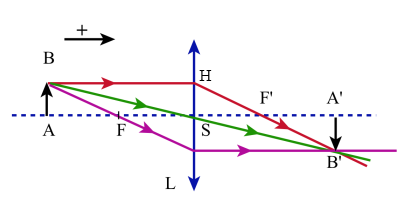
\includegraphics[scale=4]{montageSilberman}\\
On pose : 
$$
\begin{aligned}
\gamma = \dfrac{\overline{A'B'}}{\overline{AB}} ,\quad y=\overline{AA'},\quad p=\overline{SA},\quad p'=\overline{SA'},\quad \phi=\overline{SF'}=\overline{FS}
\end{aligned}
$$
Montrons que $y=-\phi\dfrac{{(\gamma-1)}^2}{\gamma}$:
\begin{multicols}{2}
	\begingroup
	\addtolength{\jot}{1em}
	\noindent
	\begin{align*}
	\dfrac{1}{p'}-\dfrac{1}{p}&=\dfrac{1}{\phi}\quad \text{relation de conjugaison}\\
\iff	p'&=\dfrac{p\phi}{p+\phi}\\
	p'-p &= \dfrac{p\phi}{p+\phi}-p\\
	y &= \dfrac{p\phi-p(p+\phi)}{p+\phi}\\
	y&=-\dfrac{p^2}{p+\phi}
	\end{align*}
	\endgroup
	\setlength\columnseprule{0.4pt}
	\vfill
	\columnbreak
	D'autre part en appliquant le théorème de Thalès aux triangle SHF' et F'A'B':
	\begingroup
	\addtolength{\jot}{1em}
	\noindent
	\begin{align*}
	\gamma&\equiv\dfrac{\overline{A'B'}}{\overline{AB}} = \dfrac{\overline{A'B'}}{\overline{SH}}\\
	&=\dfrac{\overline{A'F'}}{\overline{SF'}}\\
	&=\dfrac{\overline{A'S}+\overline{SF'}}{\overline{SF'}}\\
	&=\dfrac{-p'}{\phi}+1\\
	\iff p' &= -\phi(\gamma-1)
	\end{align*}
	\endgroup
\end{multicols}
\vspace*{+1em}
De plus on sait que : $\dfrac {\overline {AB}} {p}=\dfrac {\overline {A'B'}} {p'}\implies\dfrac{p'}{p}=\gamma$, ainsi :
\begin{empheq}[left=\empheqlbrace]{align}
	y&=-\dfrac{p^2}{p+\phi}\\
	p' &= -\phi(\gamma-1)\\
	\dfrac{p'}{p}&=\gamma
\end{empheq}
En combinant (2) et (3), on obtient : $p=\dfrac{-\phi(\gamma - 1)}{\gamma}$. On injecte dans (1) :
\begingroup
\addtolength{\jot}{1em}
\begin{align*}
	y&=-\dfrac{p^2}{p+\phi}\\
	 &=\dfrac{\left( \phi\dfrac{\gamma-1}{\gamma}\right)^2}{\left(\phi\dfrac{\gamma-1}{\gamma}\right) -\dfrac{\phi \gamma}{\gamma}}\\
	 &=\dfrac{\phi^2(\gamma-1)^2}{\gamma^2\dfrac{\phi}{\gamma}(\gamma-1-\gamma)}\\
	 &=\dfrac{-\phi(\gamma-1)^2}{\gamma}
\end{align*}
\endgroup
On a alors : $y=\dfrac{-\phi(\gamma-1)^2}{\gamma}$\\
\item 
Étudions le comportement de la fonction $y(\gamma)$ en supposant $\phi>0$ (lentille convergente). Pour le tracer de la courbe, on pose $\phi=1$, on a alors :
\begin{figure}[h]
	\centering
	\caption[]{y($\gamma$)}
	\label{fig:graphy}
	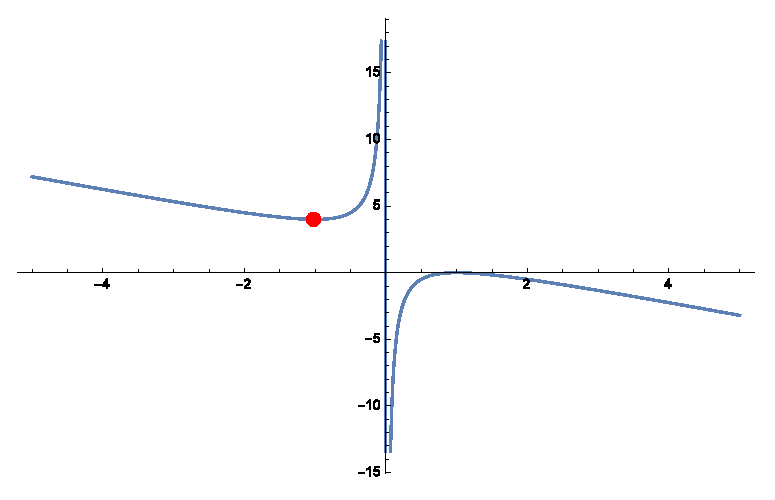
\includegraphics[scale=1.1]{images/GraphY}
\end{figure}
La fonction admet un minimum en $\gamma=-1$.\\
Étudions la fonction plus en détails. On pose $y'\equiv\dfrac {\partial y} {\partial \gamma }$ et $y''\equiv\dfrac {\partial^2 y} {\partial \gamma^2 }$. Montrons que la fonction admet un minimum en -1 :
\begin{multicols}{2}
	Recherche d'extremum : $y'=0$.\\
	Avec $\phi>0$
	\begin{align*}
	y'&=\left(\frac{1}{\gamma ^2}-1\right) \phi\\
	\end{align*}
	$y'$ s'annule en -1 et 1.
	\setlength\columnseprule{0.4pt}
	\columnbreak
	\\
	Montrons que -1 est un \textsc{Minimum} en étudiant le signe de $y''$:
	\begin{align*}
		y''&=-\dfrac{2}{\gamma^3}\\
		y''(-1)&=2>0
	\end{align*}
\end{multicols}
\vspace*{+1em}
On a $y'(-1)=0 \quad \text{et} \quad y''(-1)>2$, donc -1 est un minimum.\\
\item Si on se place dans le cas $\gamma=-1$, $y=4\phi$\\
On en déduit alors : $\phi=\dfrac{y}{4}$
\item 
On applique cette méthode sur plusieurs lentilles en prenant en compte une incertitude sur la position de l'écran p' ($\Delta p'=$0,2cm) et une incertitude de lecture sur la position de l'objet p ($\Delta p=$0,2cm).
$$\phi=\dfrac{y}{4}=\dfrac{p'-p}{4}\implies \Delta \phi = \dfrac{\sqrt{\Delta p^2+\Delta p'^2}}{4}=7.10^{-2}$$
\begin{center}

\begin{tabular}{|c|c|c|}
	\hline 
	Lentille n & $\phi_{th}$ (cm) & $\phi_{exp}$ (cm) \\ 
	\hline 
	1 & 12,7 & 12,25$\pm7.10^{-2}$ \\ 
	\hline 
	2 & 30 & 30$\pm7.10^{-2}$ \\ 
	\hline 
	3 & 20 & 19,6$\pm7.10^{-2}$ \\ 
	\hline 
\end{tabular} 
\end{center}
Les valeurs trouvées expérimentalement sont relativement proches de celles inscrites sur les lentilles.
\end{enumerate}
\subsection{Méthode de Bessel}
\section{Aberrations}
L'étude des aberrations s'effectue en utilisant des lentilles convergentes ayant une courbure importante
\subsection{Aberration sphérique}
On propose une étude qualitative de cette aberration géométrique en effectuant un relevé de points mettant en évidence l'existence de la caustique. On étudie la nappe tangentielle en relevant le diamètre de l'image en fonction de l'éloignement de l'écran.
\begin{center}
	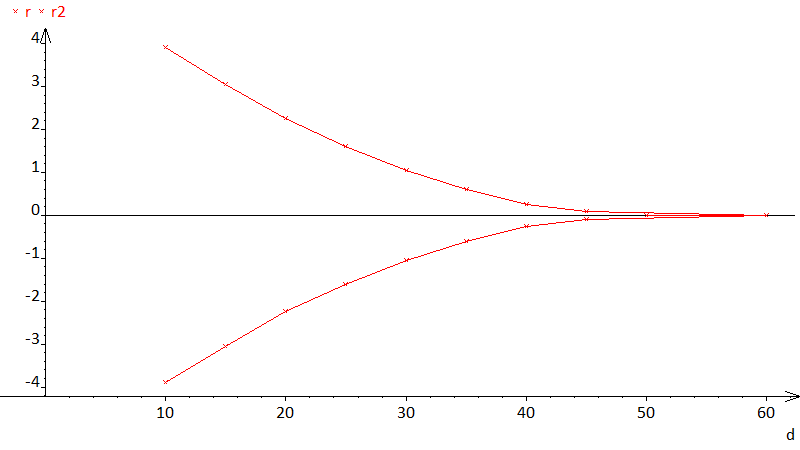
\includegraphics[scale=0.5]{images/caustique}
\end{center}
On retrouve bien la forme de caractéristique de l'aberration sphérique.
\subsection{Aberration chromatique}
Pour pouvoir observer le phénomène d'aberration chromatique, on cherche a faire l'image d'un trou à travers un lentille. convergente. On fixe l'objet et la lentille et on déplace l'écran le long de l'axe optique jusqu'à trouver le foyer. C'est alors que l'on met en évidence l'aberration chromatique puisqu'il n'existe plus un foyer unique. On distingue très clairement dans notre cas un foyer bleu puis un foyer rouge plus éloigné de la lentille. Ce phénomène s'explique car la courbure de la lentille est telle que l'on peut l'assimiler à un prisme pour les rayons les plus éloignés de l'axe optique.\\
On nous a donné $n=A+\dfrac{B}{\lambda^2}\implies$l'indice dépend de la longueur d'onde et les petites longueur d'onde sont plus déviées (milieu plus réfringent au petit n). Or on sait que :
\begin{align*}
\lambda_{bleu}(\approx400nm)&<\lambda_{rouge}(\approx800nm)\\
\implies n_{bleu}&>n_{rouge}
\end{align*}
\end{document}
